\chapter{Sistema de actores}

En este capítulo se explica cómo funciona la estructura computacional en el modelo de actores. En la primera sección se introduce el funcionamiento de las comunicaciones y el comportamiento de los actores. En la segunda sección se define la sintaxis de un lenguaje mínimo de actores, para terminar con algunos ejemplos utilizando este lenguaje.

\section{Describiendo un sistema de actores}
Un sistema de actores, consiste en configuraciones. Una configuración viene dada por una colección de actores concurrentes y una colección de comunicaciones en tránsito. Cada actor tiene un nombre único y un comportamiento. Se comunica con otros actores a través de mensajes asíncronos. Los actores son reactivos, es decir, se ejecutan solo en respuesta a los mensajes recibidos. El comportamiento de un actor es determinista, ya que la respuesta está determinada por el contenido del mensaje que procesa. 

Los actores están dados por una dirección de buzón y un comportamiento. Las comunicaciones están definidas por el par buzón destino y mensaje, de la siguiente forma:

\newcommand{\COMUNICACIONES}{\mathcal{K}}
\newcommand{\COMUNICACION}{\bar{k}}
\newcommand{\BUZONES}{\mathcal{B}}
\newcommand{\BUZONESSUB}{\mathsf{B}}
\newcommand{\BUZON}{\mathsf{b}}
\newcommand{\MENSAJES}{\mathcal{M}}
\newcommand{\MENSAJE}{\mathsf{m}}

\newcommand{\ACTOR}{\alpha}
\newcommand{\COMPORTAMIENTOS}{\mathcal{C}}
\newcommand{\COMPORTAMIENTO}{\mathsf{c}}
\newcommand{\COMNOPROC}{\kappa}
\[
\COMUNICACIONES = \BUZONES \times \MENSAJES
\]
Donde $\BUZON$ es el conjunto de las direcciones buzón. $\MENSAJES$ es el conjunto de los mensajes. 

Un comportamiento es una función que dada una comunicación, crea nuevas comunicaciones, nuevos actores y define un comportamiento de reemplazo para el actor que está procesando la comunicación. La definición del comportamiento es la siguiente:
\[
\COMPORTAMIENTOS : \COMUNICACIONES \rightarrow ( \{ \COMUNICACION_1, \COMUNICACION_2, \ldots, \COMUNICACION_m \}, \{ \ACTOR_1, \ACTOR_2, \ldots, \ACTOR_n \}, \COMPORTAMIENTO )
\]

Donde: $\COMUNICACION_1, \COMUNICACION_2, \ldots, \COMUNICACION_m$ son las comunicaciones nuevas, $\ACTOR_1, \ACTOR_2, \ldots, \ACTOR_n$ son los nuevos actores creados. El comportamiento de reemplazo esta definido por $\COMPORTAMIENTO$.

Es necesario vincular las direcciones de buzones con un determinado comportamiento. Se usa una función parcial que tiene como dominio las dirección de buzón, y como codominio los comportamientos asociados a este buzón. La definición de la función esta dada por:

\[
f_{actor} : \BUZONESSUB \rightarrow \COMPORTAMIENTOS
\]

Donde $\BUZONESSUB$ es subconjunto de $\BUZONES$ y $\COMPORTAMIENTOS$ el conjunto de los comportamientos. Esta función modela los actores que fueron creados, ya que un actor no es más que una dirección de buzón y su comportamiento.

Con estas definiciones se establece a una configuración como la tupla $(f_{actor}, \COMNOPROC)$. La evolución de un sistema de actores ocurre cuando una comunicación es procesada, es decir, que se pasa de una configuración a otra configuración.

Para que el sistema evolucione de una configuración a otra, los siguientes pasos están involucrados:
\begin{itemize}
 \item Es necesario tomar un elemento (y removerlo) del conjunto de las comunicaciones no procesadas. 
 \item La comunicación sera de la forma $(\BUZON, \MENSAJE)$, donde $\BUZON$ es buzón destino y $\MENSAJE$ un mensaje. 
 \item Al aplicar $\BUZON$ en $f_{actor}$, obtendremos el comportamiento $\COMPORTAMIENTO_b$. 
 \item Al aplicar en el comportamiento $\COMUNICACION$ el mensaje anterior $\MENSAJE$, se obtendrán los nuevos actores, los nuevos mensajes, y el comportamiento de reemplazo.
 \item A los nuevos actores se los agrega en $f_{actor}$. 
 \item Se incorporan las nuevas comunicaciones en $\COMNOPROC$. 
 \item Se tiene que cambiar en $f_{actor}$ el comportamiento de reemplazo obtenido: $\COMPORTAMIENTO_b'$. Se hace lo siguiente:  $f'_{actor} = ( f_{actor} \setminus \{ \BUZON \rightarrow \COMPORTAMIENTO_b \}) \cup \{ \BUZON \rightarrow \COMPORTAMIENTO'_b \})$. Es decir, en la nueva función de comportamientos se reemplaza para el buzón $\BUZON$ el comportamiento $\COMPORTAMIENTO_b$ por el comportamiento $\COMPORTAMIENTO'_b$.
\end{itemize} 

Estos pasos muestran cómo un sistema de actores va de una configuración a otra. 

\subsection{Comunicaciones}

Se puede decir que las \textit{Comunicaciones} que no son fueron procesadas son quienes mueven los cálculos en un sistema de actores. Las \textit{Comunicaciones} vienen representados por el par:

\begin{enumerate}
\item \textit{destino}, la dirección de buzón a la que será entregada la comunicación. 
\item \textit{mensaje}, básicamente la información que estará disponible al actor que procesará la comunicación.
\end{enumerate}

Un \textit{mensaje} es una lista de valores. Estos valores son: direcciones de buzón, enteros, cadenas de caracteres, etc. 

El \textit{destino} debe ser una dirección de buzón válida, es decir, un actor antes de enviarle una comunicación a otro actor debe tener la dirección de buzón destino, y esta debe ser valida. Existen tres formas en la cual un actor $\ACTOR$, al aceptar una comunicación $\COMUNICACION$, puede conocer la dirección de buzón de otro actor. Las formas son las siguientes:

\begin{itemize}
 \item El \textit{destino} era conocido por el actor $\ACTOR$, antes de aceptar la comunicación.
 \item El \textit{destino} estaba incluido como parte de la comunicación $\COMUNICACION$.
 \item El \textit{destino} es una dirección de buzón creada como resultado de aceptar la comunicación $\COMUNICACION$.
\end{itemize}

Es probable que más de un actor al mismo tiempo quiera enviar una comunicación a un buzón. Para esto es necesario alguna estructura intermedia que guarde todas las comunicaciones creadas y que aún no fueron procesadas. Esta estructura tiene que tener la capacidad para guardar todas las comunicaciones hasta ser procesadas por el actor destino. 

%En realidad Agha\ [chap.~3,p.~35]\cite{Agha:1986:AMC:7929} lo define como una 3-tupla incluye un \textit{tag} para diferenciar una tarea de la otra en el sistema. Define que un \textit{tag} puede tener una representación arbitraria. Como los \textit{tag} son únicos en todo el sistema, hace uso de esta propiedad para construir la direcciones de buzón de los nuevos actores creados esto puede verse en \cite[chap.~5,p.~104]{Agha:1986:AMC:7929}. 

% En el modelo que se presentará esto no es necesario.
% Otro de los argumentos sobre incluir este \textit{tag} esta relacionado con tener trazabilidad, como diferenciar dos tareas que tienen el mismo destino y la misma comunicación. En este trabajo podriamos incluir un numero aleatorio para permitir tener esta trazabilidad si quisieramos diferenciar estas dos tareas \textit{destino} y la misma \textit{comunicación}, pero se decidió dejarlo fuera.

\subsection{Actores}

Como vimos en la sección anterior toda computación en el modelo de actores es resultado de procesar comunicaciones. Un actor acepta un mensaje cuando este es procesado. Un actor sólo puede procesar comunicaciones que están dirigidas a su dirección de buzón. Como resultado de aceptar una comunicación, un actor puede: crear nuevas comunicaciones, crear nuevos actores y debe definir su comportamiento de reemplazo.

%Para un actor, el orden de llegada de las comunicaciones enviadas a ese actor debe ser lineal. Esto quiere decir el buzón debería tener algún mecanismo de \textit{buffer} para las comunicaciones que lleguen casi al mismo tiempo. 

Un actor puede describirse especificando:

\begin{itemize}
 \item Su dirección de buzón, a la que le corresponde un \textit{buzón} lo suficientemente grande para almacenar las comunicaciones aún no procesadas.
 \item Su \textit{comportamiento}, que es una función que, tiene la comunicación que está siendo procesada como entrada y como salida nuevos actores, nuevos trabajos y su nuevo comportamiento de reemplazo.
\end{itemize}

Podemos pensar que un actor es un \textit{buzón} donde llegan todas las comunicaciones, y un proceso que ejecutará su comportamiento. Este proceso apunta a una celda particular de este \textit{buzón}. 

% \begin{figure}[H]
% \begin{tikzpicture}
% 
% \draw (0,0) -- (7,0);
% \draw (0,1) -- (7,1);
% 
% \draw (0,0) -- (0,1);
% \draw (0.5,0) -- (0.5,1);
% \draw (1,0) -- (1,1);
% 
% \draw (5,0) -- (5,1);
% \draw (5.5,0) -- (5.5,1);
% 
% \node at (0.9,1.2) {$1\quad2\quad\ldots$};
% 
% \node at (5.25,1.2) {$n$};
% 
% \node at (7.8,0.5) {comunicaciones sin procesar};
% 
% \node at (6.4,-1.4) {proceso};
% 
% \draw[->] (5.25,-1) -- (5.25,0);
% \node at (5.25,-1.4) [circle,draw] (x) {$X$};

% \end{tikzpicture}
% \caption{Representación de un actor. El proceso tiene la información de su comportamiento. Acepta la comunicación actual y no puede procesar ningún otra comunicación.}
% \label{fig:mailqueue}
% \end{figure}

Cuando el proceso $X_n$ acepta la $(n)-\acute{e}sima$ comunicación, eventualmente crea el proceso $X_{n+1}$ el cual ejecutará el comportamiento de reemplazo definido por $X_n$. Este nuevo proceso apunta a la siguiente celda en el buzón en donde estará guardada la comunicación $(n+1)-\acute{e}sima$. Esto puede verse en la figura \ref{fig:actortransition}

\begin{figure}[H]
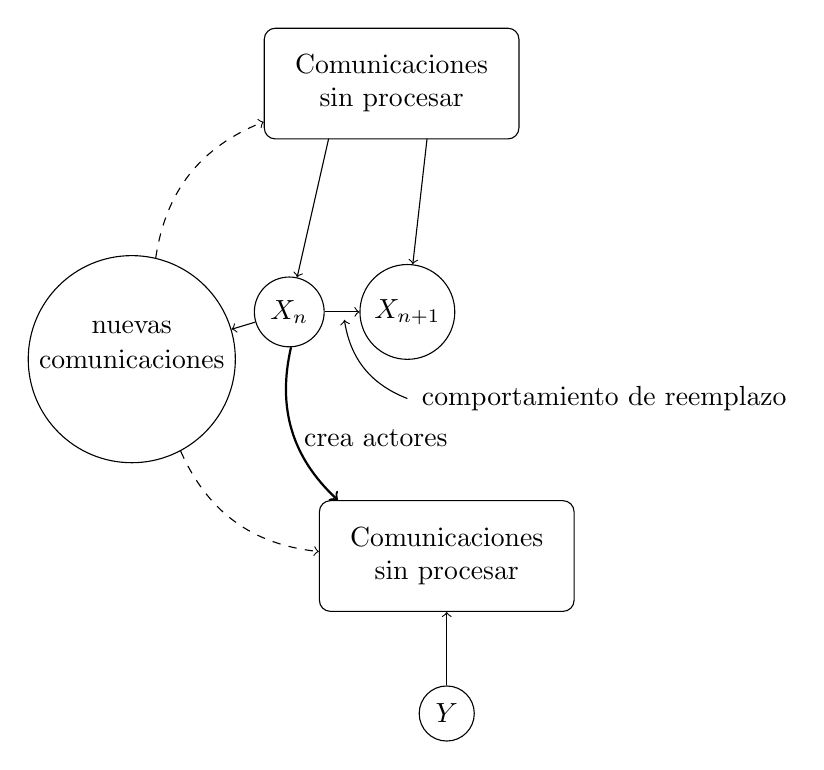
\begin{tikzpicture}
\tikzstyle{block} = [rectangle, draw, text width=3cm, text centered, rounded corners, minimum height=4em,font=\normalsize]

\node at (4,-2.4) [circle,draw] (XN) {$X_n$};
\draw[<-] (XN) -- (4.5,-.2);

\node at (5.5,-2.4) [circle,draw] (XN1) {$X_{n+1}$};
\draw[<-] (XN1) -- (5.75,-.2);

\draw[->] (XN) -- (XN1);

\node at (2,-2.6) {nuevas};
\node at (2,-3) [circle,draw] (K) {comunicaciones};



\draw[->] (XN) -- (K);

\node at (8,-3.5) {comportamiento de reemplazo};

\draw[->] (5.5,-3.5) to[bend left] (4.7,-2.5); 
\node[block, draw] (C1) at (5.3,0.5) {Comunicaciones sin procesar};

\node[block, draw] (C2) at (6,-5.5) {Comunicaciones sin procesar};

\draw[->, thick] (XN) to[bend right] (C2);
\node at (5.1,-4) {crea actores};

\node[below of=C2,yshift=-1cm, circle,draw] (Y) {$Y$};

\draw[->] (Y) -- (C2.south);

\draw[->, dashed] (K) to[bend left] (C1);
\draw[->, dashed] (K) to[bend right] (C2);


\end{tikzpicture}
\caption{Una transición entre dos comportamientos}
\label{fig:actortransition}
\end{figure}

Los dos procesos $X_n$ y $X_{n+1}$ no interfieren entre sí, pero la creación de $X_{n+1}$ depende de que $X_{n}$ haya definido su comportamiento de reemplazo. $X_n$ solo procesa la $(n)-\acute{e}sima$ comunicación. Exceptuando el caso en el cual se envíe una comunicación a si mismo. Cada uno de estos procesos crean sus propias tareas, sus propios actores como esta definido en sus comportamientos. Antes que el proceso $X_n$ cree el proceso $X_{n+1}$, $X_n$ podría haber creado otros actores u otros trabajos. Es posible incluso, que $X_n$ esté creando actores o trabajos al mismo tiempo que lo está haciendo $X_{n+1}$. Es importante notar que $X_n$ no recibirá ninguna otra comunicación, ni tampoco especificará ningún otro comportamiento de reemplazo.

% Si definimos que la creación de un actor, la creación de una tarea o especificar el comportamiento de reemplazo son eventos. El orden en que se generan estos eventos debido a que se acepto una comunicación define un orden parcial. El reemplazo de los procesos definen un orden total entre ellos. 

Esto parecería definir algún tipo de orden con respecto a cómo se van a procesar los mensajes. En el trabajo de Agha\cite{Agha:1986:AMC:7929} no se define ningún orden específico sobre el procesamiento de comunicaciones. La única garantía que tiene sobre las comunicaciones, está relacionada con el eventual proceso de los mensajes. Tanto la implementación de Erlang\cite{Cesarini:2009:EP:1717841} como la implementación de Akka\cite{Wyatt:2013:AC:2663429}, entregarán al menos una vez la comunicación a un actor, lo cual no garantiza la entrega.

%Alguna implementación puede esperar que el proceso anterior termine, para construir el nuevo y eliminar el viejo. Sin embargo, retrasar el reemplazo hasta que el proceso pueda ser reemplazado no es un requisito. Si hay suficientes recursos disponibles, la computación en un sistema de actores se puede acelerar simplemente aceptando la próxima comunicación ni bien su comportamiento de reemplazo este establecido.

\begin{figure}[H]
\centering

\tikzstyle{circulo}=[circle,draw=black, fill=black, inner sep=0pt,minimum size=3pt]
\tikzstyle{new}=[-latex, draw, dashed]
\tikzstyle{msg}=[-latex, draw]

\begin{subfigure}{.5\textwidth}
\centering
\begin{tikzpicture}[node distance=2cm]

\node[] (A) {$Actor_1$};
\node[circulo, below of=A] (A1) {};
\node[below of=A1] (A2) {};
\draw (A) -- (A2);

\node[below of=A, right of=A, yshift=1cm] (B) {$Actor_2$};
\node[circulo, below of=A, right of=A] (B1) {};
\node[below of=B1] (B2) {};
\draw (B1) -- (B2);


%\path[msg] (-1/2,-1/2) to [bend right] node[font=\small, left] {$[42]$}  (A1) ;

%\path[new] (A1) to [bend left] node[font=\small, above] {$[7]$} (B1) ;
%\path[new] (A1) to [bend right] node[font=\small, below, pos=0.6] {$[8,9]$} (C1) ;

\path[msg] (-1/2,-1/2) to [bend right] (A1) ;

\path[new] (A1) to [bend left] (B1) ;

\end{tikzpicture}

\caption{  }
\label{fig:actores:crecion:a}
\end{subfigure}%
\begin{subfigure}{.5\textwidth}

\centering
\begin{tikzpicture}[node distance=2cm]

\tikzstyle{circulo}=[circle,draw=black, fill=black, inner sep=0pt,minimum size=3pt]

\node[] (A) {$Actor_1$};
\node[circulo, below of=A] (A1) {};
\node[below of=A1] (A2) {};
\draw (A) -- (A2);

\node[right of=A] (B) {$Actor_2$};
\node[circulo, below of=A, right of=A] (B1) {};
\node[below of=B1] (B2) {};
\draw (B) -- (B2);

\node[right of=B1, yshift=1cm] (C) {$Actor_3$};
\node[circulo, right of=B1] (C1) {};
\node[below of=C1] (C2) {};
\draw (C1) -- (C2);

%\path[msg] (-1/2,-1/2) to [bend right] node[font=\small, left] {$[43]$}  (A1) ;

%\path[msg] (A1) to [bend left] node[font=\small, above] {$[1,2]$} (B1) ;
%\path[new] (B1) to [bend left] node[font=\small, above] {$[3,4]$} (C1) ;

\path[msg] (-1/2,-1/2) to [bend right] (A1) ;
\path[msg] (A1) to [bend left] (B1) ;
\path[new] (B1) to [bend left] (C1) ;

\end{tikzpicture}

\caption{}
\label{fig:actores:crecion:b}
\end{subfigure}

\caption{Las lineas verticales indican el paso del tiempo, las de punto indican creación de actores y las otras flechas envío de mensaje.}
\label{fig:actores:crecion}
\end{figure}

Como se puede ver en la figura \ref{fig:actores:crecion} \subref{fig:actores:crecion:a}, el actor $Actor_1$ recibe una comunicación. Al procesar esta comunicación, crea el actor $Actor_2$. En la figura \ref{fig:actores:crecion} \subref{fig:actores:crecion:b} se puede ver un ejemplo similar donde $Actor_1$ recibe una comunicación, como resultado envía una comunicación a $Actor_2$ y este último crea $Actor_3$.


\section{Programando con actores}\label{actores:sal}

En esta sección se explora un lenguaje que implementa los conceptos básicos del modelo de actores. 

El lenguaje \SAL fue desarrollado con intensiones pedagógicas y tiene una sintaxis heredada de Algol. En la configuración de un sistema actores, necesitamos crear actores y enviar comunicaciones. Un programa en un sistema de actores esta compuesto por:

\begin{itemize}
 \item \textit{definición de comportamientos}: asocia un esquema de comportamiento con un identificador, no crea ningún actor.
 \item expresiones \textit{new} para crear nuevos actores.
 \item comandos \textit{send} para crear nuevas tareas.
\end{itemize}

Primero se explora la sintaxis de las expresiones, ya que las expresiones son utilizadas tanto por la definición de comportamientos como por los comandos. Luego se presentará como definir comportamientos. Para terminar esta sección mostrando la definición de comandos.

%Se utilizará la notación \textbf{Backus-Naur}\cite{McCracken:2003:BF:1074100.1074155} para describir la gramática. Adjunto a la notación se utilizá el símbolo $\langle \textbf{*} \rangle$ representa una o ninguna ocurrencias de un termino. También se utilizará $\langle \textbf{+} \rangle$ para representar que haya al menos una ocurrencia.

Se utiliza la notación \textbf{Backus-Naur}\cite{McCracken:2003:BF:1074100.1074155} para describir la gramática. Adjunto a la notación se utiliza el símbolo $\langle \textbf{+} \rangle$ cuando haya al menos una ocurrencia de un término.

\subsection{Expresiones}\label{actores:exp}
Existen cuatro tipos primitivos: booleanos, enteros, cadenas, y dirección del buzón. Las operaciones posibles entre los booleanos son \textbf{or}, \textbf{and} y \textbf{not}. Los enteros se pueden operar utilizando \textbf{+}, \textbf{-}, \textbf{*} y \textbf{/}. Las cadenas son constantes. La dirección de un buzón es un identificador que es devuelto cuando se crea un nuevo actor, este tipo primitivo no tiene ningún operador asociado.

La gramática de las expresiones booleanas es la siguiente:

\begin{grammar}

<bexp> ::= <bterm> `or' <bterm> | <bterm> `and' <bterm> | <exp> = <exp>
  
<bterm> ::= <bool> | `not' <bterm> | `(' <bexp> `)' 

<bool> ::= `TRUE' | `FALSE'

\end{grammar}

La gramática de los enteros es la siguiente:

\begin{grammar}

<iexp> ::= <iterm> `*' <iterm> | <iterm> `/' <iterm> 
\alt <iterm> `+' <iterm>  | <iterm> `-' <iterm>

<número> ::= `1' | `2' | `3' | `4' | `5' | `6' | `7' | `8' | `9' | `0'

<iterm> ::= <número>$^{+}$ | `-' <iterm> | `(' <iexp> `)'

\end{grammar}

La gramática para las cadenas es la siguiente:

\begin{grammar}
 <sexp> ::= `"' <carácter>$^{+}$ `"'
\end{grammar}

Donde: \textit{carácter} es simplemente cualquier carácter entre la $A$ y la $Z$ tanto mayúscula como minúscula.

La gramática de todas las expresiones viene dada por:

\begin{grammar}
<exp> :: = <iexp> | <bexp> | <sexp> | <mexp>  
\end{grammar}

En el caso de $mexp$, es simplemente cualquier carácter entre la $A$ y la $Z$ tanto mayúscula como minúscula y representa los identificador es la dirección de buzón.

\subsection{Definición de comportamientos}\label{actores:beha}
Cada vez que un actor acepta una comunicación, define un comportamiento de reemplazo. Cada comportamiento está parametrizado. Por ejemplo, si el comportamiento de una cuenta bancaria depende de su saldo. Entonces se especifica el comportamiento de la cuenta como una función de su saldo. Cada vez que se crea una cuenta, o se define un comportamiento de reemplazo, que usa la definición de una cuenta bancaria, se tiene que dar un valor específico de saldo.

Existen dos listas de parámetros que están involucradas en la definición de un comportamiento. La primera lista corresponde a los parámetros que son dados al momento de la creación de un actor, esta lista es llamada \textit{acquaintance-list}. La segunda, que se obtiene cuando una comunicación es aceptada, es llamada \textit{comunication-list}.

En el caso de la lista de identificadores \textit{communication-list}, esta asume que todas las comunicaciones serán una secuencia de identificadores. Supongamos el siguiente caso: un comportamiento que modela una cuenta bancaria. Resulta útil que esta lista de identificadores esté dada en función de la operación que se vaya a ejecutar, por ejemplo, si la operación fuera \textit{`extracción'} solamente necesitaríamos un identificador \textit{`monto'} el cual tendría el valor de la extracción en cuestión. En el caso que la operación fuera \textit{`balance'} esta no requiere identificadores. 

Se presenta a continuación una gramática que contempla el caso en cual \textit{communication-list} sea sólo una lista de identificadores (se verá mas adelante en el ejemplo del calculo del factorial). También se presenta una forma de bifurcación ante diferentes ramas dependiendo del contenido de la comunicación (el ejemplo de la una pila hace uso de esto). La gramática de los comportamientos es la siguiente:

\begin{grammar}
<BDef> :== `def' $NombreComportamiento$ `(' <acquaiantence-list> `)' <body> `end def'

<acquaiantence-list> :== <id> | <id> `,' <acquaiantence-list> 

<body> :== <static-list> | <match-list>

<static-list> :== `[`'<comunication-list>`]' \\ <command>

<comunication-list> :== <id> | <id> `,' <comunication-list>

<match-list> :==  `match' ( `case' `[' <case-list> `]:' <command> )+  

<case-list> :== <case-exp> | <case-exp> `,' <case-list> 

<case-exp> :== <bool> | <numero> | <id>  
\end{grammar}
Donde: 

\begin{description}
 \item $NombreComportamiento$ identifica un comportamiento. Tiene alcance a todo el programa. 
 \item \textit{static-list} son completados al momento de procesar una comunicación, y su alcance es todo \textit{command}. 
 \item \textit{comunication-list} se utiliza para definir una lista de identificadores.
 \item \textit{case-exp} puede ser de tipo booleana, un número o un identificador. 
 \item \textit{case-list} se utiliza para definir una lista de elementos de tipo \textit{case-exp}.
 \item \textit{match-list} Se comparan las expresiones una a una, de haber coincidencia se ejecutan los comandos que están a continuación. De contener identificadores libres, estos se inicializarán con el valor contenido en el mensaje para esa posición.
 \item \textit{acquaiantence-list} los recibe al momento de inicialización y tiene alcance en todo \textit{command}.
 \item \textit{body} puede ser una lista de argumentos estática o se puede utilizar el operador \textit{match}. En la siguiente sección se define \textit{command}.
\end{description}

Ambas listas, \textit{comunication-list} y \textit{acquaiantence-list}, contienen todos los identificadores libres que están en \textit{command}. En el caso de \textit{match-list} los identificadores libres tienen alcance a los \textit{commands} asociado a cada \textit{case}. Existe un identificador especial \textit{self} que puede ser utilizado para hacer referencia al buzón del actor que se está definiendo. 

La ejecución de \textit{command} deberá contar a lo sumo con un solo comando \textit{become}, esta propiedad tiene que ser garantizada de manera estática, de no existir ningún comando \textit{become}, el actor asumirá un comportamiento de tipo \textit{bottom}, que es básicamente ignorar los mensajes que se le envíen.

\subsection{Definición de comandos}\label{actores:cmd}
Los comandos son las acciones que permite a \SAL crear nuevos actores, enviar mensajes y definir un nuevo comportamiento. Estos describen en esencia lo que un actor puede hacer dentro de un comportamiento.

Command viene definido definido por la siguiente gramática:
\begin{grammar}
<command> :== <A> | <B> | <C> | <D>
\end{grammar}

Donde: $A$, $B$, $C$ y $D$ se definen en las próximas secciones.

\subsubsection*{Creando actores}
Los actores son creados usando expresiones de tipo \textit{new}, que devuelve una nueva dirección de buzón del actor recién creado. La sintaxis de las expresiones de tipo \textit{new} es la siguiente:

\begin{grammar}
  <expr_list> ::= <exp> | <exp> `,' <expr_list>  

  <new_expr_list> ::= <new_expr> | <new_expr> `,' <new_expr_list>
  
  <new_expr> ::= $mexp$ `=' `new' $NombreComportamiento$ `(' <expr_list> `)'
  
  <A> ::=  `let' <new_expr_list> `in' <command> 
\end{grammar}

$NombreComportamiento$ hace referencia a un identificador vinculado con un comportamiento específico, declarado utilizando una \textit{definición de comportamiento}. Se crea un nuevo actor con el comportamiento descripto en la definición del comportamiento y sus parámetros son instanciados con los valores de las expresiones entre paréntesis. Utilizando el léxico de actores, corresponde a los valores denominados como \textit{acquaintance-list}. El identificador $mexp$ es el valor de la dirección del buzón. Este identificador puede ser destino de nuevas comunicaciones. 

Los actores son creados de manera concurrente, estos pueden conocer entre sí la dirección de buzón. Esta es una forma de definición mutuamente recursiva que es perfectamente válida en el modelo de actores. 

%En todo actor recientemente creado lo único que el actor que esta creando un nuevo sabe de este es su dirección de buzón, es decir, no tiene ningún acceso a la estructura interna del actor creado.

\subsubsection*{Creando comunicaciones}
Una comunicación es creada especificando un actor destino y un mensaje. Las comunicaciones se pueden enviar a actores que ya fueron creados o actores creados por quien está enviando la comunicación. El destino es la dirección de buzón del actor al que le queremos enviar la comunicación. La sintaxis de este comando podría ser la siguiente:

\begin{grammar}
  <B> ::= `send' `[' <expr_list> `]' `to' <mexp>  
\end{grammar}

Donde $expr\_list$ es una lista de expresiones, que puede ser vacía. Las expresiones son evaluadas y se envían los valores en la comunicación. $mexp$ es un identificador que tiene asociado una dirección de buzón de un actor. 

\subsubsection*{Comportamiento de reemplazo}

El propósito de los comandos es especificar las acciones que pueden ocurrir. Se mostraron los comandos para crear nuevos actores y para crear nuevas tareas. También se necesita un comando para definir el comportamiento de reemplazo. La sintaxis para este último tiene la forma:

\begin{grammar}
  <C> ::= `become' $NombreComportamiento$ `(' <expr_list> `)'
  \alt `become' $mexp$
\end{grammar}

También se puede utilizar el identificador de un comportamiento, especificando los parámetros \textit{acquaiantence-list}. Donde $mexp$ es una dirección de buzón, en este caso reenvía todos los mensajes al nuevo buzón.  Por ejemplo:

\begin{align*}
 \texttt{become}&\ link \\
 \texttt{become}&\ Comp(1,2,3) 
\end{align*}

Donde $link$ es alguna dirección de buzón, y $Comp(1,2,3)$ hace referencia al comportamiento $Comp$, y su \textit{acquaiantence-list} son los valores $1$, $2$ y $3$. La sintaxis del comportamiento se describe en la sección \ref{actores:beha}

\subsubsection*{Otros comandos}

Para completar el lenguaje, se agregan la composición secuencial y un condicional.

\begin{grammar}
  <D> :== `if` <bexp> `then' <command> `else' <command> `end if'
  \alt <command> ; <command>
\end{grammar}

donde:

\begin{description}
\item [if-then-else], después de evaluar la expresión booleana, si es verdadera
  ejecuta lo que esta a continuación de \textbf{then}, en caso contrario lo que está a
  continuación de \textbf{else}. Funciona como cualquier condicional.
\item [composición] Dos comandos que se ejecutan de manera secuencial.

\end{description}

\section{Ejemplos}

En esta sección mostraremos dos ejemplos escritos en \SAL y algunas particularidades del lenguaje. Primero se presenta el código del ejemplo, a continuación una breve descripción linea por linea de la funcionalidad, y para terminar se mencionan notas sobre su funcionamiento.

\subsection{Cálculo del factorial}\label{sal:factorial}

Se usa este clásico ejemplo, para mostrar que el paso de mensaje se puede usar como una estructura de control. En un lenguaje imperativo una función recursiva está implementada utilizando una Pila de llamadas. Usar esta pila, implica que factorial solo puede procesar un único cálculo a la vez, una vez que termina el cálculo puede aceptar nuevamente otro. En los lenguajes secuenciales no existe ningún mecanismo que permita distribuir el calculo del factorial o que permita concurrentemente procesar más de una petición.

La implementación utilizando el modelo de actores depende de crear uno o más trabajadores que están a la espera de la respuesta adecuada. El actor factorial está dispuesto a procesar concurrentemente la próxima comunicación. Esta incluye la dirección de buzón a cual se debe enviar el calculo del factorial.

Está implementación del factorial está adaptada de \cite{Agha:1986:AMC:7929}. Depende de un actor \lstinline[language=sal, style=simple]$Main$ que envía al actor \lstinline[language=sal, style=simple]$Factorial$ el valor a calcular, en el caso del ejemplo: el valor $3$. La palabra reservada \textit{self} hace referencia a este buzón, correspondiente al actor que está procesando la comunicación.

Como se observa en el ejemplo, las comunicaciones pueden venir tanto del actor \lstinline[language=sal, style=simple]$Main$ como del actor \lstinline[language=sal, style=simple]$Factorial$.

\begin{lstlisting}[language=sal, style=simple]
def Factorial()[val, customer]
  if val = 0 then
    send [1] to customer
  else
    let cont = new FactorialWorker(val, customer)
       in send [val - 1, cont] to self
  end if 
  become Factorial()
end def

def FactorialWorker(n, customer)[m] 
  send [n * m] to customer
end def

def Main() 
  let fact = new Factorial() 
    in send [3, self] to fact
end
\end{lstlisting}

\begin{description}

\item [Línea 1] $Factorial$ no recibe ningún parámetro en el momento de ser inicializado, pero sí recibe dos parámetros cuando procesa una comunicación, la lista $[val, customer]$ con un entero y una la dirección de un buzón respectivamente.
\item [Línea 3] Envía una lista con el valor $1$ al actor con buzón $customer$.
\item [Línea 5] Crea un actor de tipo FactorialWorker. En este caso se utiliza $new$, ya que se está creando un nuevo buzón, y éste se asigna a la variable $cont$. Cuando se asigna el nuevo comportamiento, éste recibe los parámetros $val$ y $customer$.
\item [Línea 6] Envía un mensaje a la dirección del buzón propio utilizando la palabra reservada $self$, con la lista $val - 1$ y la dirección del buzón que se acaba de crear.
\item [Línea 8] Asigna como siguiente comportamiento a $Factorial()$, sin parámetros ya que $Factorial$ no recibe ningún parámetro a la inicialización.  
\item [Línea 11] FactorialWorker recibe dos valores cuando es instanciado: un entero $n$ y la dirección de un buzón $customer$. Cuando procesa un mensaje, en su \textit{acquaiantence-list} recibe un entero $m$.
\item [Línea 12] Envía la multiplicación $n*m$ como lista a la dirección del buzón $customer$ 
\item [Líneas 15-18] Inicializa el actor $Factorial$ y le envía a este la lista con los valores $3$ y la dirección del buzón actual. 

\end{description}

Concretamente, el actor ante un entero distinto de cero ejecuta dos acciones, crea un actor que espera un mensaje con un número y multiplica este número por \textbf{n}, luego se envía el resultado al buzón de $customer$.

También, se envía un mensaje a sí mismo para evaluar el factorial de \textbf{n - 1}, y como dirección de cliente utiliza la dirección del buzón del actor recientemente creado. Es decir, el resultado de $fact(n - 1)$ se le pasará al actor recientemente creado que lo multiplicará por $n$.

Esto establece una red de actores que multiplican el valor indicado y enviarán el cálculo al siguiente actor en la red, es el último actor en la red el que lo enviará a quien originalmente lo pidió.

En la figura \ref{fig:factorial} se puede ver que el actor $Factorial()$ recibe como comunicación la lista $[3,c]$, esto hace que ocurran dos cosas:

\begin{itemize}
\item Se cree un actor nuevo $FactorialWorker$ con buzón $c1$, este recibe dos parámetros en la inicialización: el valor $3$ y el buzón inicial que recibió como comunicación, es decir quien pidió originalmente la computación del factorial de $3$.

\item Se envíe a sí mismo el mensaje $[2,c1]$, este inicia el cálculo del factorial de $2$, es decir el cálculo de $fact(n-1)$, el paso recursivo.
\end{itemize}

Ahora $c1$ es quien pide el calculo del factorial de $2$. Esto se repite hasta que el valor a calcular el factorial de $0$.

Cuando el primer elemento de la comunicación es cero, hace que se le envíe al actor cuya dirección de buzón fue recién recibida, la lista con el valor uno. 

\begin{itemize}
\item $a$ le envía el valor $1$ a $c3$.
\item $c3$ multiplica $1*1$ y se lo envía a $c2$.
\item $c2$ multiplica $2*1$ y se lo envía a $c1$.
\item $c1$ multiplica $3*2$ y se lo envía a $c$.
\end{itemize}

Recordamos que $c$ había pedido el calculo del factorial $3$ en primer lugar.

\begin{figure}[H]
\centering
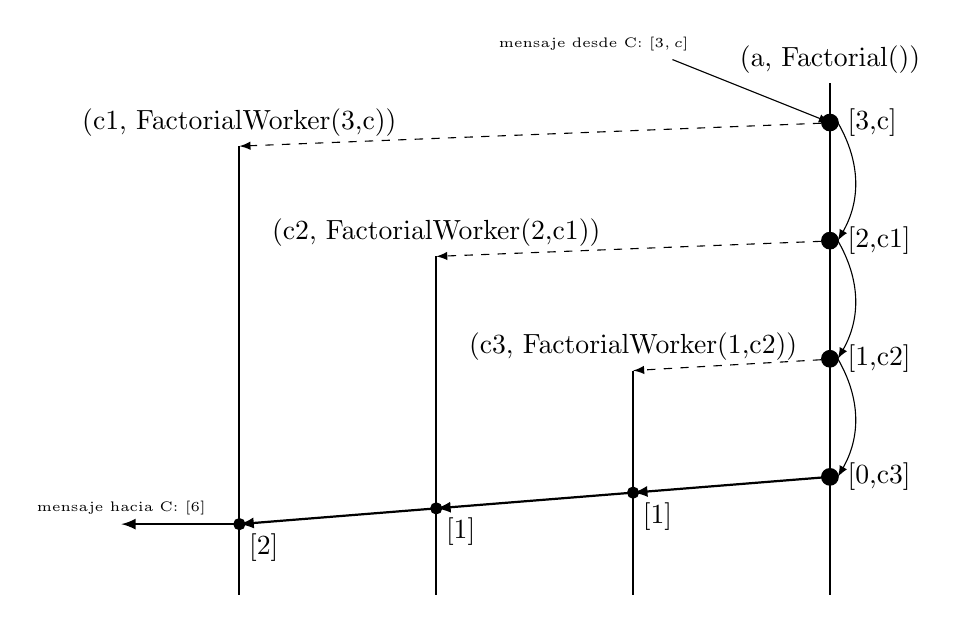
\begin{tikzpicture}

\draw[-latex] (6,7.3) to (8,6.5);

\draw[thick] (8,7) -- (8, 0.5);

\node[] at (5,7.5) {\tiny mensaje desde C: $[3,c]$};

\node[] (a1) at (8,7.3) {(a, Factorial())};

\node[align=center, right] (a1) at (8.1,6.5) {[3,c]};
\draw[fill] (8,6.5) circle (3pt);

\node[align=center, right] (a2) at (8.1,5) {[2,c1]};
\draw[fill] (8,5) circle (3pt);

\node[align=center, right] (a3) at (8.1,3.5) {[1,c2]};
\draw[fill] (8,3.5) circle (3pt);

\node[align=center, right] (a4) at (8.1,2) {[0,c3]};
\draw[fill] (8,2) circle (3pt);

\draw[-latex] (a1.west) to[bend left] (a2.west);
\draw[-latex] (a2.west) to[bend left] (a3.west);
\draw[-latex] (a3.west) to[bend left] (a4.west);

\node[] (d1) at (0.5,6.5) {(c1, FactorialWorker(3,c))};
\draw[thick] (d1.south) -- (0.5, 0.5);

\node[] (c1) at (3,5.1) {(c2, FactorialWorker(2,c1))};
\draw[thick] (c1.south) -- (3, 0.5);

\node[] (b1) at (5.5,3.65) {(c3, FactorialWorker(1,c2))};
\draw[thick] (b1.south) -- (5.5, 0.5);

\draw[fill] (5.5,1.8) circle (2pt);
\node[align=center, right] (b2) at (5.5,1.5) {[1]};

\draw[fill] (3,1.6) circle (2pt);
\node[align=center, right] (c2) at (3,1.3) {[1]};

\draw[fill] (0.5,1.4) circle (2pt);
\node[align=center, right] (d2) at (0.5,1.1) {[2]};

\draw[-latex, thick] (8,2)  -- (5.5,1.8);
\draw[-latex, thick] (5.5,1.8) -- (3,1.6);
\draw[-latex, thick] (3,1.6) -- (0.5,1.4);
\draw[-latex, thick] (0.5,1.4) -- (-1,1.4);

\draw[-latex, black, dashed] (a1.west) -- (d1.south);
\draw[-latex, black, dashed] (a2.west) -- (c1.south);
\draw[-latex, black, dashed] (a3.west) -- (b1.south);

\node[] at (-1,1.6) {\tiny mensaje hacia C: $[6]$};

\end{tikzpicture}

\caption{El diagrama ilustra el cálculo del factorial de 3, todo el resultado es enviado al actor \textit{c}. Las líneas verticales indican el paso del tiempo, las de punto indican creación de actores y las otras flechas envío de mensaje. La lista superior indica  dirección del buzón, tipo de actor con los parámetros de inicialización.}

\label{fig:factorial}

\end{figure}

\subsection{Una pila usando actores}\label{sal:pila}

Otro ejemplo que podemos encontrar en \cite{Agha:1986:AMC:7929} es el de una pila, que está representada con una lista enlazada. Se utiliza la dirección de un buzón, como un puntero a un nodo de esta lista. 

Tiene dos operaciones básicas: apilar ($push$), que coloca un nodo en la pila, y su operación inversa, sacar ($pop$), que remueve el último elemento agregado en la pila.

\begin{lstlisting}[language=sal, style=simple]
def Node(content, link)
  case ['pop', customer]:
    send content to customer;
    become link;
  case ['push', newcontent]:
    let P = new node(content, link)
      in become node(newcontent, P)
end def

def Main() 
  let stack = new node(10, Nil)
    in send [push, 20] to stack;
       send [push, 30] to stack;
  end
end
\end{lstlisting}

\begin{description}

\item [Línea 1] $Node$ recibe dos parámetros, $content$ que es un entero, el valor que tiene que guardar el nodo y  $link$ es una dirección de buzón, es el siguiente actor en la pila.
\item [Línea 2] Si la operación es $'pop'$, guarda en $customer$ la dirección de buzón.
\item [Línea 3] Envía el contenido del nodo a la dirección de buzón $customer$
\item [Línea 4] La instrucción $become$, en este caso, hace que se reenvíen todos los mensajes a la dirección de buzón $link$. 
\item [Línea 5] Si la operación es $'push'$, guarda en $newcontent$ el valor del entero recibido.
\item [Línea 6] Crea un nuevo actor con los parámetros de inicialización $content$ y $link$.
\item [Línea 7] Asigna el siguiente comportamiento, como $node$ con los parámetros $newcontent$ y la dirección de buzón del actor recién creado $P$. 
\item [Líneas 11-13] Crea una nueva pila con uno nodo con valor $10$, y envía dos operaciones $push$ con los valores $20$ y $30$.
\end{description}

El comportamiento $node$ funciona como una lista enlazada, donde en vez de tener direcciones de memoria tenemos direcciones de buzón. El primer parámetro es el contenido a guardar $content$ y el segundo $link$ es el actor siguiente en la pila, el puntero al siguiente elemento.

Cuando $operation$ es de tipo $pop$, se envía el valor que contiene el nodo al buzón $customer$ y se reenvían todos los mensajes a $link$, todas las futuras operaciones $push$ y $pop$ las recibe este nodo, es decir que ahora es la ``cabeza'' de la pila. Esto guarda un parecido a mover un ``puntero''.

Cuando $operation$ es de tipo $push$, la pila crea un nuevo $node$ que será el nodo que quedará siguiente en la red, se puede ver que esto ocurre en las líneas 7 y 8. Se copia en $P$ el nodo actual, y crea un nuevo nodo que es la nueva ``cabeza''.

Puede observarse en el ejemplo, que el primer nodo creado tiene como valor $Nil$, esto es simplemente una referencia nula. 

